\chapter{Related Work}

% Describe very broadly other approaches to embedding documents. What has been
% achieved rather than how some methods work.

% Current shortcomings:

% \begin{enumerate}

%   \item minimal resources about teacher-student (de-facto only SBERT)

%   \item few papers dedicated strictly to embedding documents

%   \item Add Lora

% \end{enumerate}

In this chapter we go over the research that we consider relevant to the
embedding of long pieces of text. Since the goal of this thesis is to use the
transformer architecture, we first describe what are the obstacles in embedding
longer documents using transformers and how can be these obstacles overcome.
Next we talk about typical approaches to training of embedding models. Finally,
there are some ways of embedding texts that are not typical and which we would
like to mention.

\section{Efficient transformers}

% \begin{itemize}

%     \item How long inputs=documents are handled by transformers?

%     \item Why they cannot be handled by classical architectures?

%     \item What can be done for transformer to handle long texts? -- attention
%         mechanism, attention implementation, different architecture altogether

% \end{itemize}

Though the Transformer~\cite{vaswani2017attention} proved to be performant
architecture (TODO: citations) in the world of natural language processing (or
\emph{NLP}) it has one inherent disadvantage when it comes to longer sequences
of text. The self-attention, which is the principal part of the transformer
architecture, consumes quadratic amount of memory to the input length. This
significantly limits transformer's applicability to variety of tasks that
require longer contexts such as document retrieval or summarization.

There are several ways how to address this limitation. Most of them fall into
the following three categories:

\begin{enumerate}

    \item designing a new memory efficient attention mechanism,

    \item using custom attention implementation, or

    \item designing new transformer architecture altogether.

\end{enumerate}

We go over each category separately, though often these approaches can be and
sometimes are combined (TODO: at least one link).

\subsection{Attention mechanisms}

\begin{itemize}

    \item Efficient Transformers~\cite{tay2022efficient} -- nice overview of
    efficient transformers

    \item Longformer~\cite{beltagy2020longformer} -- the easiest implementation
        of sparse attention

    \item BigBird~\cite{zaheer2020big} -- has some insights both about
    sparse attentions (only cover very briefly) and about document processing, a
        bit more complex approach to attention

    \item BigBird-ETC

    \item Sparse transformer~\cite{child2019generating} -- even more complex
        attention implementation

    \item Reformer/Performer -- some other transformer that uses other method
        than just sparsifying attention pattern

    \item Transformer-XL

\end{itemize}


Designing more efficient self-attention mechanism in practice means trading of
some of the performance of standard full attention for better efficiency. There
are several methods that sacrifice performance in different ways.

\subsubsection{Sparse attention}

Classical self-attention~\cite{vaswani2017attention} computes the following
equation:

\begin{equation}
    Attnention(Q, K, V) = \text{softmax}(\frac{QK^T}{\sqrt d}) V = WV
\end{equation}

where $Q, K, V \in \mathcal{R}^{n\times d}$ are query, key and value matrices
respectively and $W \in \mathcal{R}^{n\times n}$ is a matrix of weights. Note
the matrix multiplication $QK^T$ which requires $O(n^2)$ memory. But by
zeroing-out some areas in $W$, or more concretely by not computing them both
when when multiplying $QK^T$ and $WV$ one could significantly save memory as
well as time. Such attention is typically called \emph{sparse} compared to the
classical \emph{full}. Based on what areas we leave out, the sparse attention
typically falls into one of the following categories:

\begin{itemize}

    \item \emph{local attention} -- tokens attend only to their neighbouring tokens --
        Figure~\ref{fig:attn_pattern_local},

    \item \emph{dilated local attention} -- tokens attend to their $k$-th neighbouring
        tokens -- Figure~\ref{fig:attn_pattern_dilated_local},

    \item \emph{global attention} -- tokens attend to all other tokens such as in full
        attention -- Figure~\ref{fig:attn_pattern_global},

    \item \emph{random attention} -- tokens attend to randomly chosen tokens --
        Figure~\ref{fig:attn_pattern_random}, or

    \item combination of any of the above mentioned attention patterns --
        Figure~\ref{fig:attn_pattern_combination} displays combination of
        local, global and random attentions.

\end{itemize}

Making the attention pattern more sparse is relatively easy way how to trade off
performance for efficiency. All types of attention except dilated local
attention can be efficiently implemented by splitting $Q, K$ and $V$ matrices
into blocks and do calculations separately on each block~\cite{zaheer2020big}.
Such calculation takes linear amount of memory in input length.

Typically only a subset of the sparse attention types is used for each model.
For instance Longformer~\cite{beltagy2020longformer} uses only local, dilated
local and global attentions, BigBird~\cite{zaheer2020big} uses local, random and
global attentions and Sparse Transformer~\cite{child2019generating} uses only
local, dilated local and global attentions.

\begin{figure}
\centering

    \begin{subfigure}{0.15\textwidth}
        \centering
        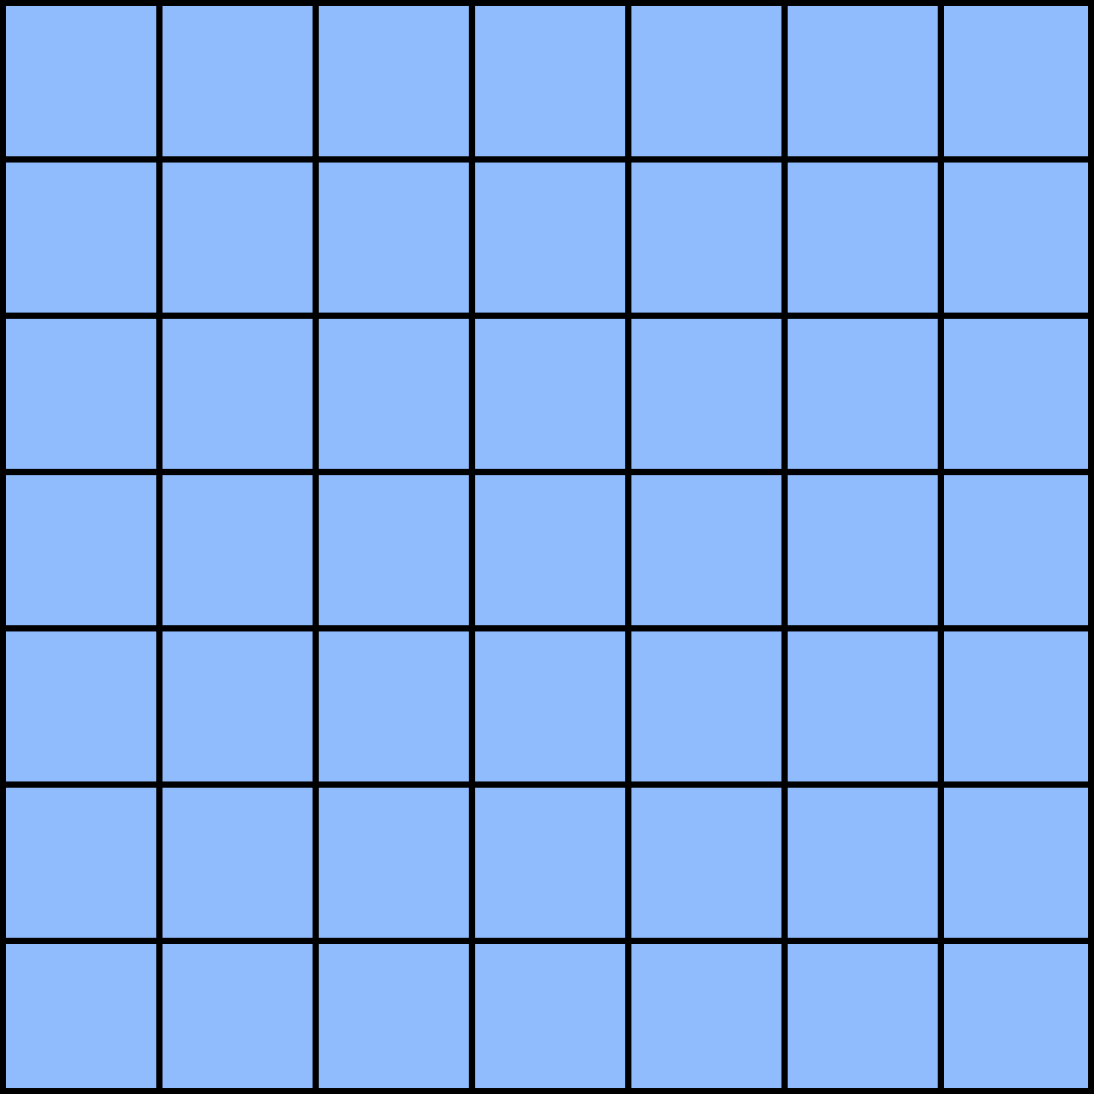
\includegraphics[width=\textwidth]{./img/full_attention.png}
        \caption{}\label{fig:attn_pattern_full}
    \end{subfigure}
    \begin{subfigure}{0.15\textwidth}
        \centering
        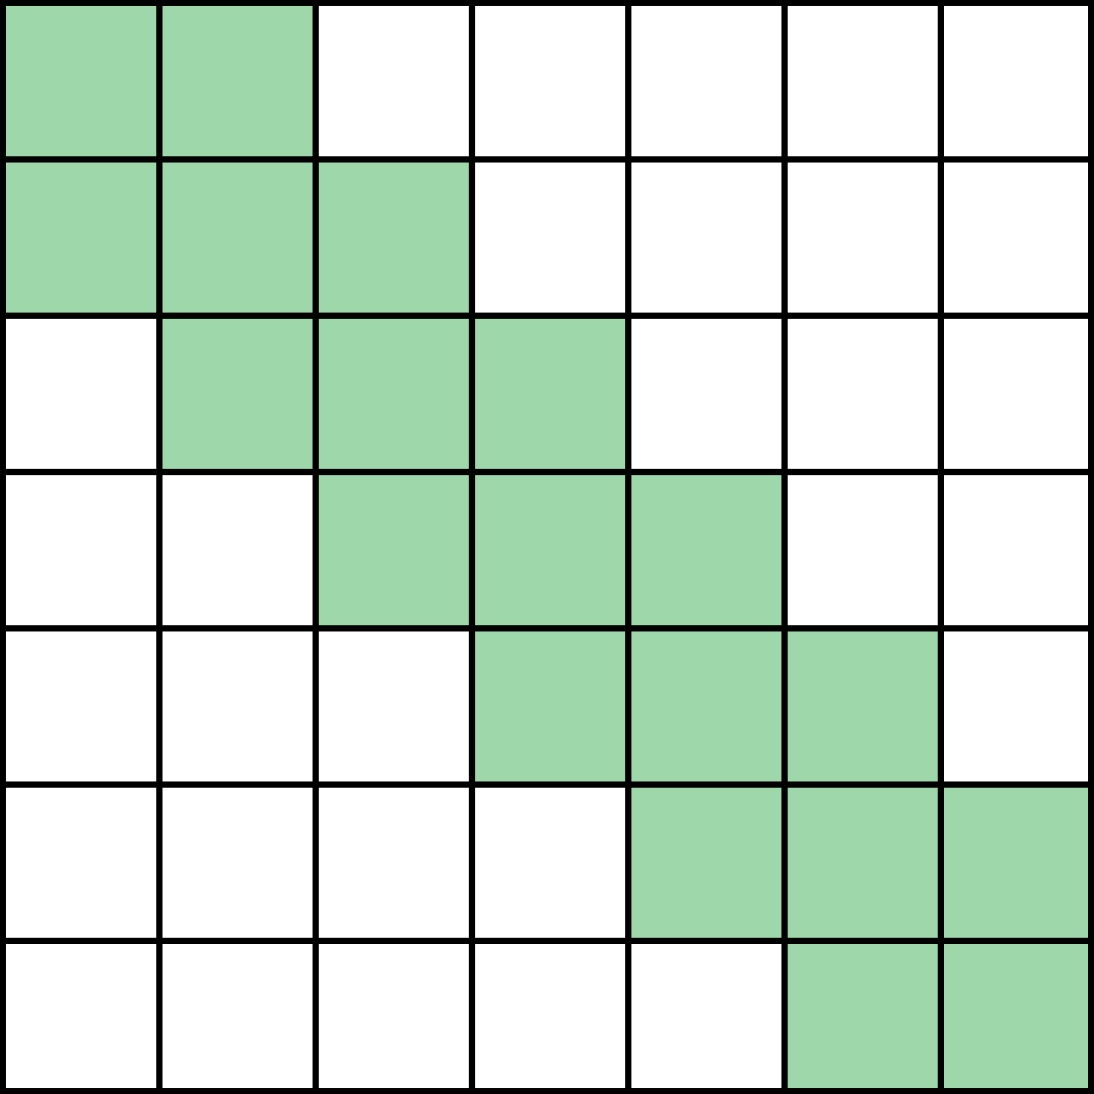
\includegraphics[width=\textwidth]{./img/local_attention.png}
        \caption{}\label{fig:attn_pattern_local}
    \end{subfigure}
    \begin{subfigure}{0.15\textwidth}
        \centering
        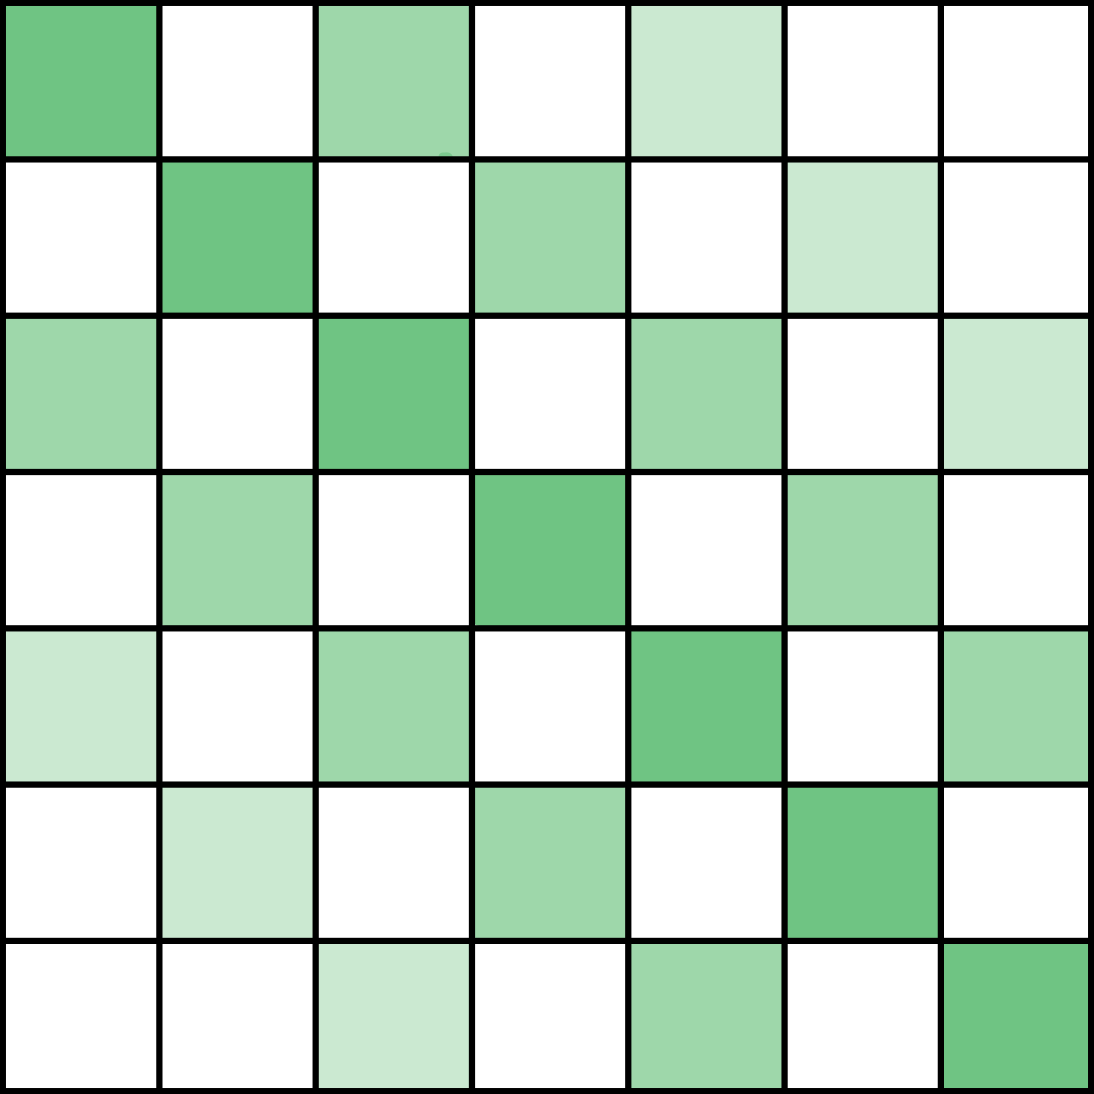
\includegraphics[width=\textwidth]{./img/local_strided_attention.png}
        \caption{}\label{fig:attn_pattern_dilated_local}
    \end{subfigure}
    \begin{subfigure}{0.15\textwidth}
        \centering
        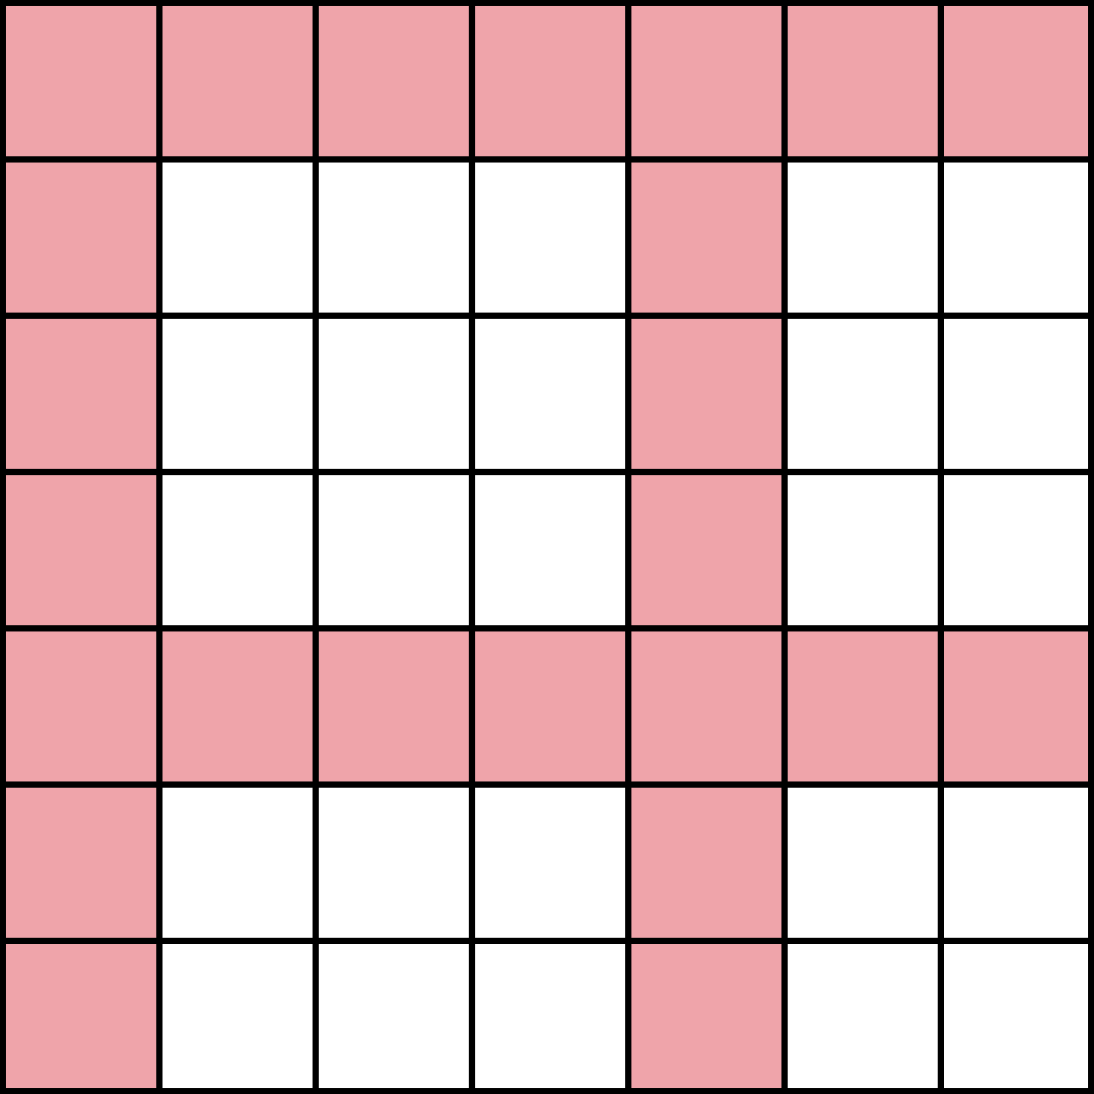
\includegraphics[width=\textwidth]{./img/global_attention.png}
        \caption{}\label{fig:attn_pattern_global}
    \end{subfigure}
    \begin{subfigure}{0.15\textwidth}
        \centering
        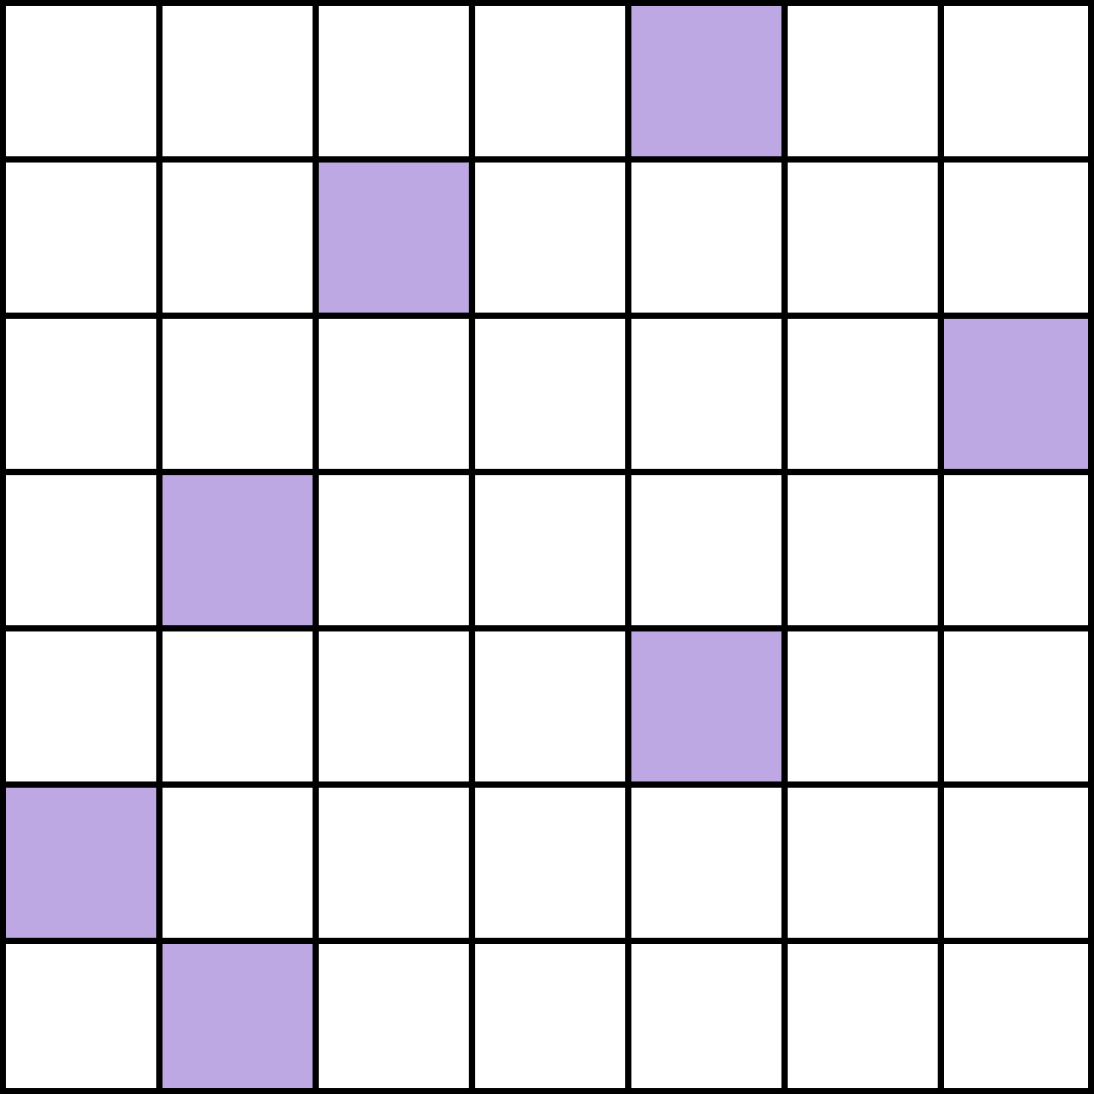
\includegraphics[width=\textwidth]{./img/random_attention.png}
        \caption{}\label{fig:attn_pattern_random}
    \end{subfigure}
    \begin{subfigure}{0.15\textwidth}
        \centering
        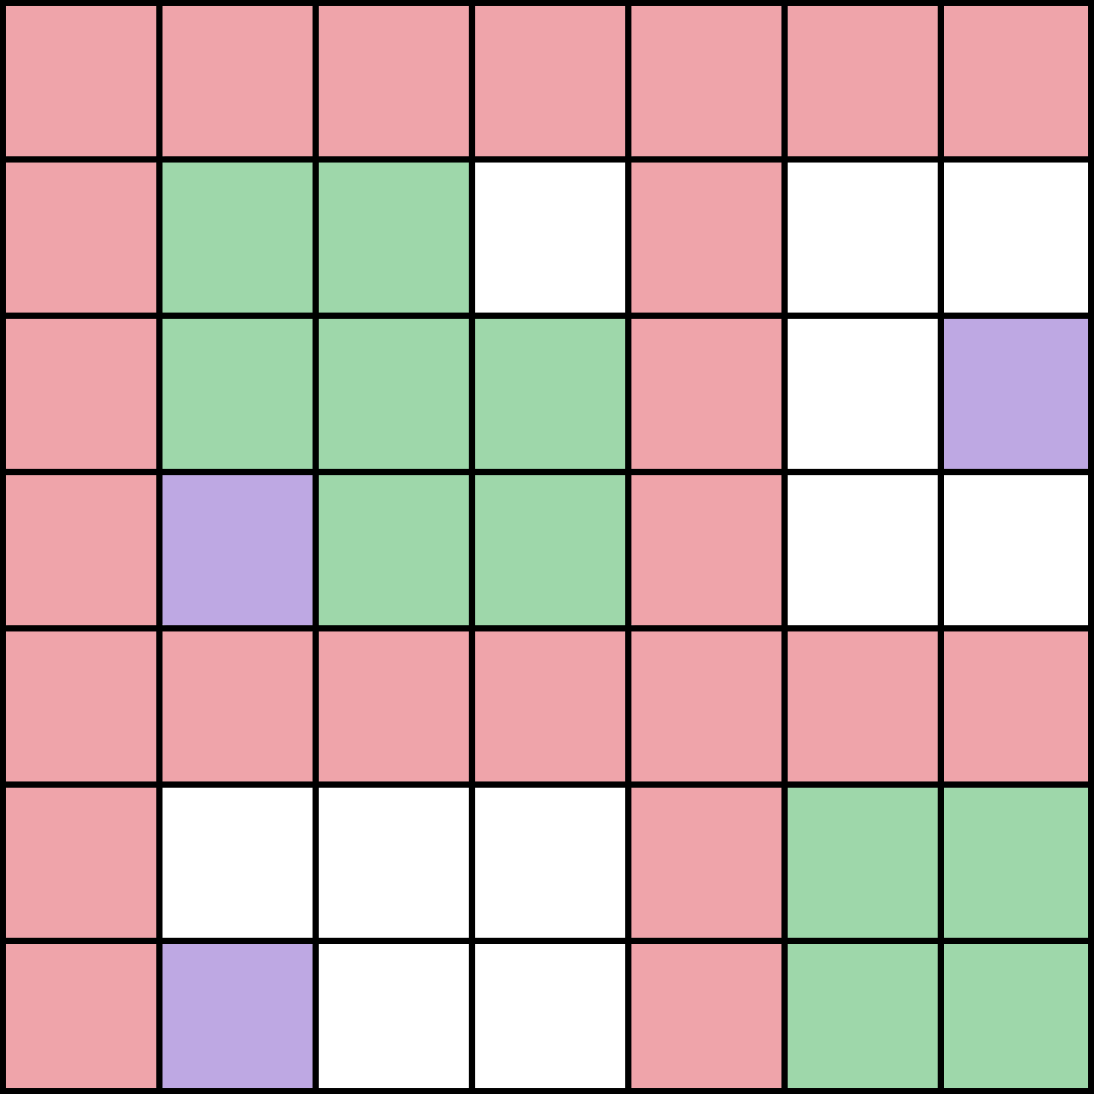
\includegraphics[width=\textwidth]{./img/mix_attention.png}
        \caption{}\label{fig:attn_pattern_combination}
    \end{subfigure}

    \caption{Self-attention patterns visualized as result of multiplication of
    query and key matrices. Colored areas are computed, while blank ones are
    not. From left to right these are called (a)~full, (b)~local, (c)~dilated
    local, (d)~global, (e)~random, and (f)~combination of local, random and
    global attentions.}\label{fig:combined}

\end{figure}

\subsubsection{}

\subsection{Attention implementation}

\begin{itemize}

    \item Flash Attention 2 -- mention it, just to show there are approaches that
    completely ditch sparse attentions (such as LLama2 Long)

    \item xFormers -- dtto

    \item Llama 2 Long -- bringing long context to the extreme, only uses full attention

\end{itemize}

\subsection{Implementation tricks}

\begin{itemize}

    \item To make the computation more effective different tricks can be used at
        the implementation level.

    \item Although these tricks can be applied to other network architectures as
        well, they are particularly useful here since they can decrease the
        memory usage by quite a lot.

    \item fp16

    \item gradient checkpointing

\end{itemize}

\subsection{Different transformer architectures}

\begin{itemize}

    \item Siamese Multi-depth Transformer-base Hierarchical (SMITH)
    encoder~\cite{yang2020beyond} -- approach to long inputs using hierarchies
    rather than changing type of attention

    \item Hierarchical Attention Network (HAN)~\cite{yang2016hierarchical} --
    hierarchical approach along text objects (words, sentences, paragraphs) for
    document classification

\end{itemize}

\section{Training approaches}

\begin{itemize}

    \item How can be (long) text embeddings trained?

\end{itemize}

\subsection{Autoregressive Language Modelling}

\begin{itemize}

    \item Standard pre-training for many transformers

    \item Paragraph Vector~\cite{le2014distributed} -- just mentioned it. It is
    already surpassed methodology.


\end{itemize}

\subsection{Siamese networks}


\begin{itemize}

      \item SBERT~\cite{reimers2019sentence} -- did pretty much the same as us
        (took a model and finetuned it so that the produced embeddings are good),
        except for sentences

      \item MPNet~\cite{song2020mpnet} -- best SBERT model and the model we are
        working with

\end{itemize}

\subsection{Knowledge distillation}

\begin{itemize}

      \item That paper where SBERT is finetuned on low-resource language with
          teacher-student training~\cite{reimers2020making}

\end{itemize}

\subsection{Contrastive loss}

\begin{itemize}

      \item OpenAI embedding paper -- use contrastive loss, mention large batches
        and the memory constraints it brings

      \item Specter~\cite{cohan2020specter} -- focused on scientific documents, use
        of contrastive loss based on citations

      \item Transformer based Multilingual document embedding
        model~\cite{li2020transformer} -- transformer version of LASER, embeds
        documents

\end{itemize}

\section{Unorthodox document embedding approaches}

\begin{itemize}

    \item Self-Supervised Document Similarity Ranking~\cite{ginzburg2021self} --
    really focused on generating semantically meaningful representations of
    documents, but with an extra cost and complexity


    \item Cross-Document Language Modelling~\cite{caciularu2021cdlm} -- uses
    Longformer for cross-document task. Illustrates that Longformer can be
    flexible and useful for document processing.

\end{itemize}
